% CE7454 Group 17 project report, CVPR 2027 author-kit format.
% Compile with pdflatex + bibtex (Overleaf default) or latexmk -pdf main.tex

\documentclass[10pt,twocolumn,letterpaper]{article}

%%%%%%%%% PAPER TYPE
% \usepackage[review]{cvpr}      % anonymous review version with line numbers
% \usepackage{cvpr}              % camera-ready, no page numbers
\usepackage[pagenumbers]{cvpr}   % class report: show authors and page numbers

% Additional packages go in preamble.tex (loaded before hyperref)
%% Packages and macros shared by main.tex. Loaded before hyperref.

\usepackage{booktabs}     % \toprule, \midrule, \bottomrule
\usepackage{multirow}
\usepackage{siunitx}      % aligned numeric columns: S[table-format=...]
\usepackage{caption}      % \captionof, caption spacing
\usepackage{xspace}

%% Inline annotations (red). Disable for the final version by uncommenting the
%% two \renewcommand lines below.
\newcommand{\red}[1]{{\color{red}#1}}
\newcommand{\todo}[1]{{\color{red}#1}}
\newcommand{\TODO}[1]{\textbf{\color{red}[TODO: #1]}}
% \renewcommand{\TODO}[1]{}
% \renewcommand{\todo}[1]{#1}

%% Dataset and method names
\newcommand{\pathmnist}{PathMNIST\xspace}
\newcommand{\dermamnist}{DermaMNIST\xspace}
\newcommand{\pneumnist}{PneumoniaMNIST\xspace}
\newcommand{\deit}{DeiT-S\xspace}
\newcommand{\pp}{pp\xspace}  % percentage points

%% Work harder in optimising text layout. Enable at the very end, when just
%% above the page limit; typically shrinks text by about 1/6 of a page.
% \usepackage{microtype}

%% Tighter paragraph headings
% \renewcommand{\paragraph}[1]{\vspace{.5em}\noindent\textbf{#1.}}

\DeclareMathOperator*{\argmin}{arg\,min}
\DeclareMathOperator*{\argmax}{arg\,max}


\definecolor{cvprblue}{rgb}{0.21,0.49,0.74}
\usepackage[pagebackref,breaklinks,colorlinks,allcolors=cvprblue]{hyperref}

\def\confName{CE7454}
\def\confYear{2026}

%%%%%%%%% TITLE
\title{How Many Tokens Does a Medical ViT Need?\\
Validation-Selected Token Reduction and Parameter-Efficient Recovery on MedMNIST}

%%%%%%%%% AUTHORS
\author{Aditya Pugalia \qquad \TODO{Author 2} \qquad \TODO{Author 3}\\
Group 17, CE7454 Deep Learning for Data Science\\
Nanyang Technological University, Singapore\\
{\tt\small adityapugalia30@gmail.com}
}

\begin{document}
\maketitle
\begin{abstract}
Vision transformers (ViTs) spend most of their compute on a fixed set of image tokens, and token-reduction methods developed on ImageNet promise large savings. Whether those savings transfer to small medical datasets, where a single missed class can matter, is unclear. We study token reduction and parameter-efficient adaptation for a \deit backbone on three MedMNIST benchmarks (\pathmnist, \dermamnist, \pneumnist) under a pre-registered protocol: budgets are chosen on validation only, test configurations are hashed and locked before any test inference, and non-inferiority is judged with conservative paired bounds rather than point estimates. Across 279 validation configurations, 90 ablations and 48 locked test evaluations we find that (i) the tolerable reduction is strongly dataset-dependent, from 90\% of tokens on \pathmnist to 25\% on \dermamnist; (ii) attention-guided deletion is not reliably better than random deletion; (iii) ToMe-style merging extends tolerance far beyond deletion on two datasets; and (iv) despite small mean losses, \emph{no} policy established the predeclared 0.5\,\pp non-inferiority margin on held-out test data across three seeds, while two extra epochs of recovery training shrank mean test losses to within 0.4\,\pp. We further compare full, partial, linear and LoRA fine-tuning for both initial adaptation and post-pruning recovery, measuring accuracy against trainable parameters, training time and memory. \TODO{one-sentence fine-tuning/LoRA result once the grid finishes.} Code, locked specifications and per-image predictions are released.
\end{abstract}

\section{Introduction}
\label{sec:intro}

Transformer backbones now match or exceed convolutional networks on medical image classification, but a ViT processes every $16\times16$ patch through every block regardless of content~\cite{dosovitskiy2021vit,touvron2021deit}. For a $224\times224$ input this is 196 image tokens, and self-attention and feed-forward cost scale with that count. Token reduction methods such as DynamicViT~\cite{rao2021dynamicvit}, EViT~\cite{liang2022evit} and ToMe~\cite{bolya2023tome} drop or merge tokens part-way through the network and report 30--50\% throughput gains on ImageNet at under one point of accuracy loss.

Medical classification differs from ImageNet in ways that matter for these methods. Datasets are small and class-imbalanced, discriminative evidence may occupy a tiny region (a lesion, a sub-type of tissue), and a mean accuracy drop of half a point can hide a much larger drop in the recall of a clinically important class. Training sets of a few thousand images also make full fine-tuning of a 22M-parameter backbone a questionable use of compute, motivating parameter-efficient adaptation such as LoRA~\cite{hu2022lora}. Prior work on adaptive inference for medical ViTs is sparse and mostly validation-tuned~\cite{byun2026adaptive,zhou2023tokensparse}.

We ask a deliberately narrow question: \emph{for a fixed fine-tuned \deit, how many tokens can be removed after the early blocks before held-out accuracy and class recall degrade, and does the answer depend on the dataset, the reduction mechanism, the reduction depth, and whether the model is briefly re-trained?} Answering it honestly requires guarding against the optimistic bias that creeps in when a budget is chosen and reported on the same data. We therefore adopt a four-stage protocol (\cref{sec:method}): baselines with three training seeds, a validation screen over four reduction methods and five budgets, focused ablations, and a locked test confirmation in which policies and checkpoint hashes are frozen before inference and non-inferiority is assessed with conservative simultaneous paired bounds.

\paragraph{Contributions.}
\begin{itemize}
  \item A controlled comparison of random deletion, attention-guided deletion, EViT-style fusion and ToMe-style merging on three MedMNIST tasks, with 279 validation configurations and matched compute, latency and memory measurements.
  \item Ablations on reduction depth, progressive schedules and input-stage removal, showing that where tokens are removed matters more than how many.
  \item A pre-registered, locked test evaluation with paired conservative bounds. Its main finding is negative: validation-selected budgets with small mean losses did \emph{not} establish non-inferiority on test, and short recovery training only partly closes the gap.
  \item A comparison of full, partial, linear-probe and LoRA fine-tuning for initial adaptation and for post-pruning recovery, reporting accuracy together with trainable parameters, wall-clock training time and peak memory. \TODO{Refine once the grid is complete.}
\end{itemize}

\section{Related Work}
\label{sec:related}

\paragraph{Token reduction in ViTs.}
DynamicViT~\cite{rao2021dynamicvit} learns a lightweight prediction module that drops tokens at fixed depths and requires joint training with a distillation loss. A-ViT~\cite{yin2022avit} halts individual tokens adaptively. EViT~\cite{liang2022evit} ranks tokens by the class-token attention and fuses the inattentive remainder into a single token between attention and MLP. ToMe~\cite{bolya2023tome} is training-free: it bipartite-matches tokens by key similarity and merges the most similar pairs at every layer, tracking token mass through proportional attention. Zero-TPrune~\cite{wang2024zerotprune} and Token Cropr~\cite{bergner2025cropr} extend training-free pruning to attention-graph importance and to dense prediction tasks respectively. All of these are developed and evaluated on ImageNet-scale data. Our adapters are controlled simplifications of EViT and ToMe applied after a complete block (\cref{sec:method}); we do not reproduce their exact schedules, and we compare them to the two obvious baselines, random and attention-ranked deletion, under identical budgets.

\paragraph{Efficient inference for medical imaging.}
Zhou \etal~\cite{zhou2023tokensparse} sparsify tokens for medical segmentation, and Byun \etal~\cite{byun2026adaptive} study adaptive inference for medical ViT classifiers. Both select operating points on validation data; to our knowledge no prior work on medical token reduction locks its configurations before test evaluation or reports paired non-inferiority bounds~\cite{walker2011noninferiority}, which we argue is necessary because validation and test sets in MedMNIST are small and, for \pathmnist, come from different clinical centres~\cite{yang2023medmnist}.

\paragraph{Parameter-efficient fine-tuning.}
Raghu \etal~\cite{raghu2019transfusion} showed that ImageNet transfer to medical images often yields most of its benefit from the early layers, so training only the head or the last blocks can be competitive. LoRA~\cite{hu2022lora} adds low-rank updates to attention projections and is now standard for language models; its behaviour on small medical vision datasets, and in particular as a recovery mechanism after token pruning, is less studied. We compare full, partial (last-$k$-block), linear-probe and LoRA adaptation under a common efficiency accounting.

\section{Method and Protocol}
\label{sec:method}

\subsection{Backbone, data and baselines}
We fine-tune the non-distilled \deit checkpoint (\texttt{deit-small-patch16-224}: 12 blocks, width 384, 6 heads, 22M parameters)~\cite{touvron2021deit} independently on three MedMNIST~v2 tasks at $224\times224$~\cite{yang2023medmnist}: \pathmnist (9 colorectal tissue classes; 90k/10k/7.2k train/val/test), \dermamnist (7 skin lesion classes; 7.0k/1.0k/2.0k) and \pneumnist (binary chest X-ray; 4.7k/0.5k/0.6k). Official splits are kept; archives are MD5-verified. Training uses random-resized crops (scale 0.8--1.0) and horizontal flips, AdamW~\cite{loshchilov2019adamw} with learning rate $5\times10^{-5}$, weight decay 0.05, batch 32 and a cosine schedule. Epoch counts (5, 10, 5) were fixed from single-seed pilots on validation. Three seeds (0, 1, 2) are trained per dataset and the best-validation checkpoint is kept; test data never informs any choice. A loading check rejects any missing or mismatched backbone weight, since an early run that silently dropped the pretrained weights produced misleading baselines.

\subsection{Token reduction adapters}
All adapters act on the frozen fine-tuned model and physically shorten the token sequence after a complete transformer block (block 4 unless stated), keeping the class token and original positional embeddings. Budgets retain $n\in\{147, 98, 69, 49, 20\}$ of 196 image tokens, i.e.\ 25--90\% reduction. Because earlier blocks process all tokens, $n$ measures sequence length downstream of the reduction point, not total compute or discarded image content; we report measured FLOPs separately.

\textbf{Random deletion} ranks tokens with i.i.d.\ uniform scores; three mask seeds separate mask variance from training variance. \textbf{Attention deletion} keeps the top-$n$ tokens by head-averaged class-query attention from the preceding block; the cost of recomputing that row is included in profiling. \textbf{EViT-style fusion}~\cite{liang2022evit} keeps the top-$(n{-}1)$ attention-ranked tokens and replaces the rest with one attention-weighted summary that counts toward the budget. \textbf{ToMe-style merging}~\cite{bolya2023tome} repeatedly splits image tokens into alternating sets, matches by cosine similarity of block-output features, and merges the most similar pairs until $n$ remain; merged tokens carry mass, which biases later attention logits by $\log$ mass. Fusion happens after a full block rather than between attention and MLP, and merging repeats at one depth rather than at every layer, so both are controlled adaptations rather than reproductions. A no-op adapter is tested bit-exact against the original model.

\subsection{Fine-tuning and recovery methods}
\label{sec:finetune}
We compare four ways of adapting the backbone, each with a learning rate chosen on a seed-0 validation pilot: \textbf{full} ($5\times10^{-5}$), \textbf{partial} (last 4 blocks and final norm, $3\times10^{-4}$), \textbf{linear} (head only, $3\times10^{-3}$) and \textbf{LoRA}~\cite{hu2022lora} on the query and value projections ($r{=}8$, $\alpha{=}16$, dropout 0.1, $1\times10^{-3}$) via PEFT~\cite{peft}. The head is always trained. LoRA weights are merged on export so every checkpoint is a plain ViT state dict usable by the same evaluation and pruning code. For every run we record trainable parameters, optimisation-only wall-clock time, peak GPU memory, and validation accuracy four times per epoch to estimate time-to-target.

\textbf{Recovery} re-trains a pruned model for two epochs with the reduction active, starting from the fine-tuned checkpoint, at a budget one step more aggressive than the validation-selected one (floor 20 tokens). A full-token control receives the same extra training from the same checkpoint, so the recovery comparison is matched in training budget. We run recovery with full-parameter updates ($10^{-5}$) and with LoRA-only updates ($2\times10^{-4}$), and also test LoRA recovery from a LoRA-fine-tuned start, i.e.\ a parameter-efficient pipeline end to end.

\subsection{Selection, locking and confirmation}
\label{sec:protocol}
The protocol, including tolerances, seeds and the interval procedure, is written to a JSON file before the test stage. The primary tolerance is $\delta{=}0.5$\,\pp of accuracy, with 1\,\pp as a secondary margin; these are research thresholds, not clinical criteria. On validation, a method's selected budget is the most aggressive $n$ whose accuracy is within $\delta$ of the full model for \emph{every} training seed (and every mask seed for random). Ties across methods prefer more reduction, then mean accuracy, then latency. For the selected method we ablate reduction depth (after blocks 1, 4, 8), a progressive schedule (blocks 4, 7, 10 with geometrically decreasing counts) against a single-stage control matched in FLOPs, and input-stage removal before block 1 (random and uniform grid) with the full patch-embedding cost still counted.

Before any test inference, the selected policies, their specification hashes, the protocol hash and all 27 checkpoint hashes are committed to a manifest. For each fixed (reference, reduced) checkpoint pair the test accuracy difference is the fraction of images improved minus the fraction harmed. A paired image bootstrap (10{,}000 resamples) gives a descriptive 95\% interval~\cite{efron1994bootstrap}. The confirmatory statistic is a conservative lower bound: the Clopper--Pearson~\cite{clopper1934} lower bound on the improvement probability minus the upper bound on the harm probability, each at $\alpha/6$ with $\alpha{=}0.05$, which is simultaneous across the two tails and three seeds. Non-inferiority is supported only if all three seeds' bounds exceed $-\delta$~\cite{walker2011noninferiority}. Image rows are the resampling unit because MedMNIST does not expose patient identifiers.

\subsection{Efficiency measurement}
FLOPs count supported PyTorch operators at two per multiply-add and include selection, fusion and merging overhead; the image-token count entering every block is logged. Latency (batch 1) and throughput (batch 32) are medians of 30 timed forwards after 10 warm-ups on real held-out batches with device synchronisation, in float32 on an RTX PRO 6000 (Blackwell) GPU with PyTorch 2.11 and Transformers 5.20. Peak allocated memory is recorded. FLOP reduction and measured speed-up are always reported separately because they disagree.

\section{Experiments}
\label{sec:experiments}

\subsection{Baselines (Stage 1)}
\Cref{tab:baselines} reports the nine fine-tuned baselines. Seed variation is already comparable to the 0.5\,\pp tolerance on \dermamnist and \pneumnist, which is why every selection rule below is applied per seed rather than to the mean.

\begin{table}[t]
  \centering
  \small
  \begin{tabular}{lrrr}
    \toprule
    Dataset & Epochs & Val.\ acc.\ (\%) & Val.\ AUROC \\
    \midrule
    \pathmnist  & 5  & $99.85 \pm 0.03$ & 1.000 \\
    \dermamnist & 10 & $89.43 \pm 0.85$ & 0.983 \\
    \pneumnist  & 5  & $98.16 \pm 0.79$ & 0.999 \\
    \bottomrule
  \end{tabular}
  \caption{Full-parameter \deit baselines, mean $\pm$ SD over three training seeds. Validation only; test is untouched until \cref{sec:locked}.}
  \label{tab:baselines}
\end{table}

\subsection{Validation screen (Stage 2)}
\Cref{fig:screen} plots validation accuracy against retained tokens for all four methods, three seeds and, for random deletion, three masks (279 configurations). Applying the per-seed 0.5\,\pp rule gives very different budgets: \pathmnist tolerates merging down to 20 tokens (89.8\% reduction, 99.54\% vs.\ 99.85\%), \dermamnist tolerates only 147 tokens with EViT-style fusion (25\%), and \pneumnist 69 tokens with merging (64.8\%), where merging actually \emph{raised} mean validation accuracy to 98.73\%. Deletion of any kind failed to qualify on \pneumnist. At matched budgets attention ranking beat random deletion on \dermamnist but was worse on \pathmnist (99.04\% vs.\ 99.61\% at 49 tokens) and \pneumnist, so attention importance is not a safe default. EViT-style fusion was indistinguishable from plain attention deletion (e.g.\ 88.57\% vs.\ 88.60\% at 98 tokens on \dermamnist), whereas merging extended the tolerable budget substantially on two of three datasets.

\begin{figure}[t]
  \centering
  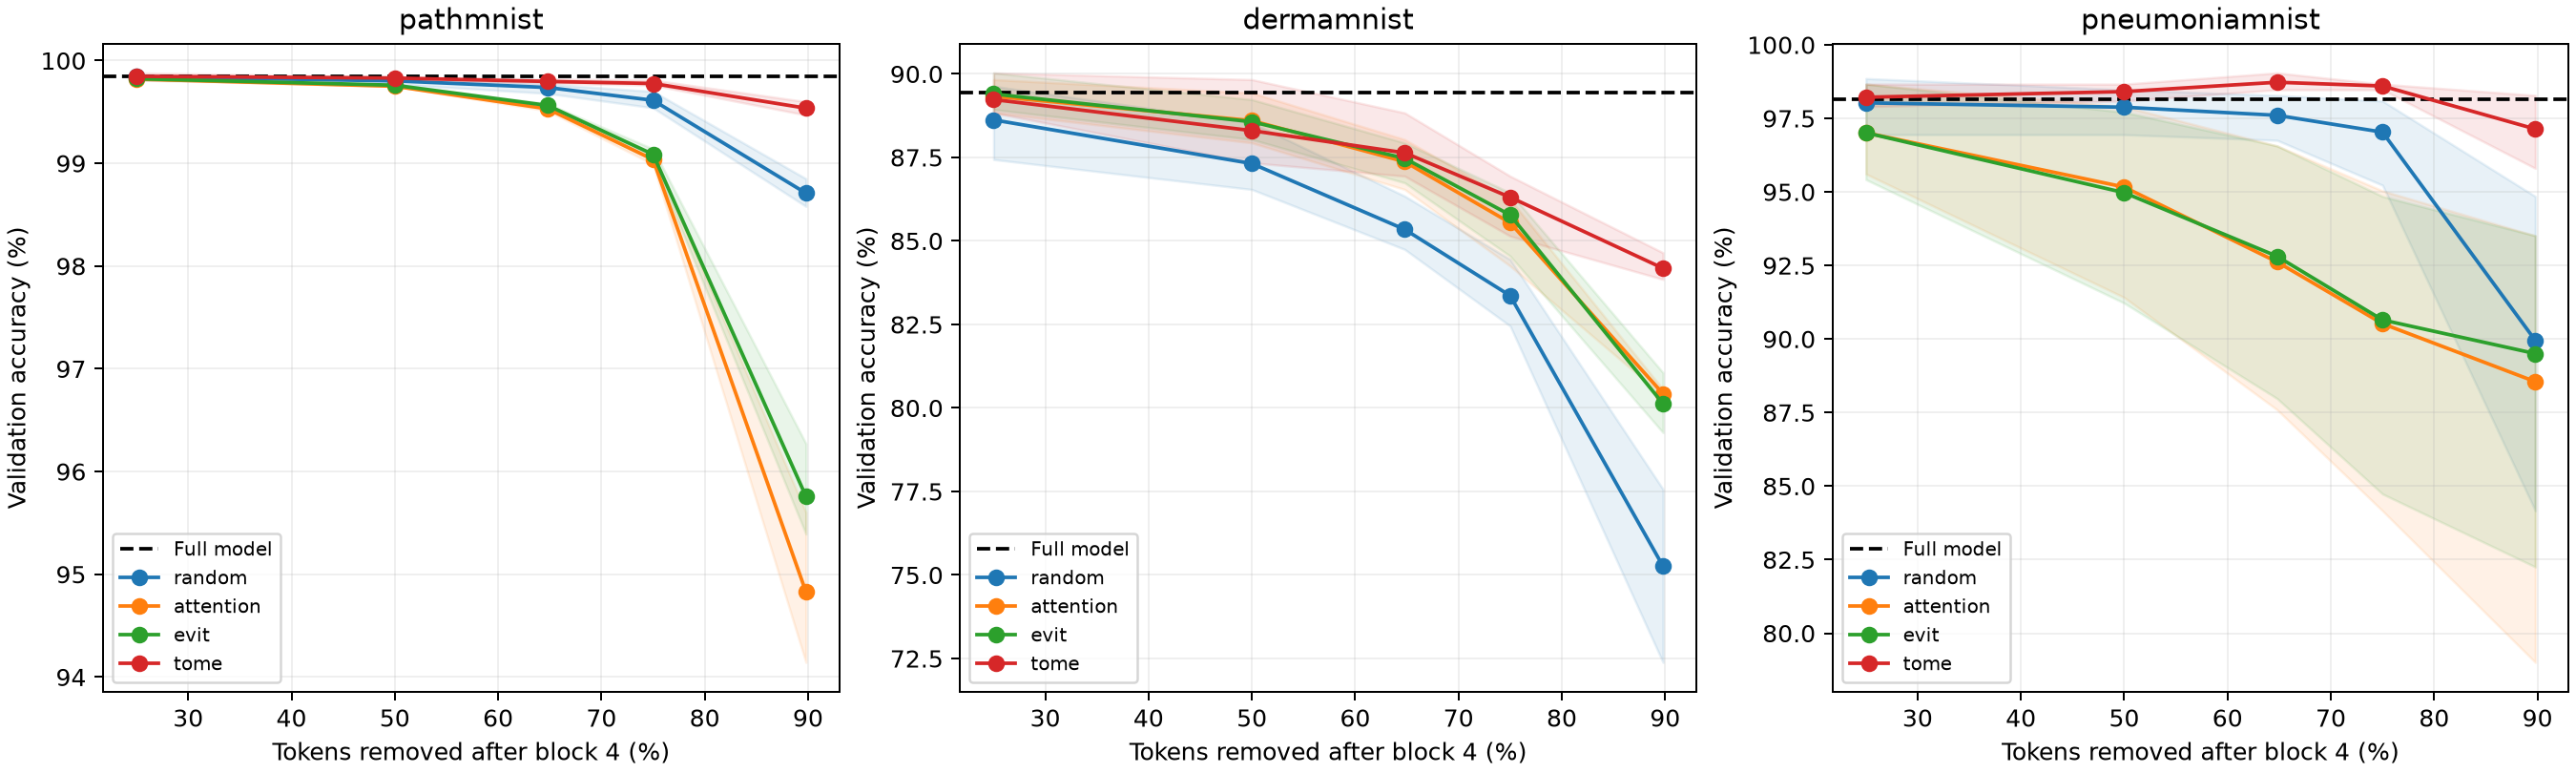
\includegraphics[width=\linewidth]{fig/accuracy_tradeoffs.png}
  \caption{Validation accuracy versus retained image tokens after block 4 for each dataset and method. Shading is the observed range across seeds and masks. Horizontal lines mark the full model and the 0.5\,\pp tolerance.}
  \label{fig:screen}
\end{figure}

\subsection{Ablations (Stage 3)}
\label{sec:ablations}
\textbf{Depth.} Merging \pathmnist to 20 tokens after block 1, 4 or 8 gives 70.4\%, 99.5\% and 99.9\% at 1.7, 3.8 and 6.5 GFLOPs (full model 9.2). The relationship is not monotonic: \pneumnist is better after block 4 (98.7\%) than block 8 (98.0\%). \textbf{Input removal} is far more damaging than intermediate reduction at the same count: keeping 20 of 196 \pathmnist patches before block 1 drops accuracy to 88.1\% (random) or 83.8\% (uniform grid), and 69 \pneumnist patches give 90.3\%. \textbf{Progressive} merging over blocks 4, 7 and 10 to 20 tokens on \pathmnist reaches 99.83\% at 4.81 GFLOPs versus 99.79\% for a single reduction to 56 tokens at 4.81 GFLOPs, but is slower at batch 1 (3.06 vs.\ 2.35\,ms), so it buys nothing on this hardware. \textbf{Recovery} (two epochs at the next-more-aggressive budget) recovers validation accuracy to within 0.1\,\pp of its matched control on all three datasets. \Cref{fig:examples} shows which patches attention deletion keeps.

\begin{figure}[t]
  \centering
  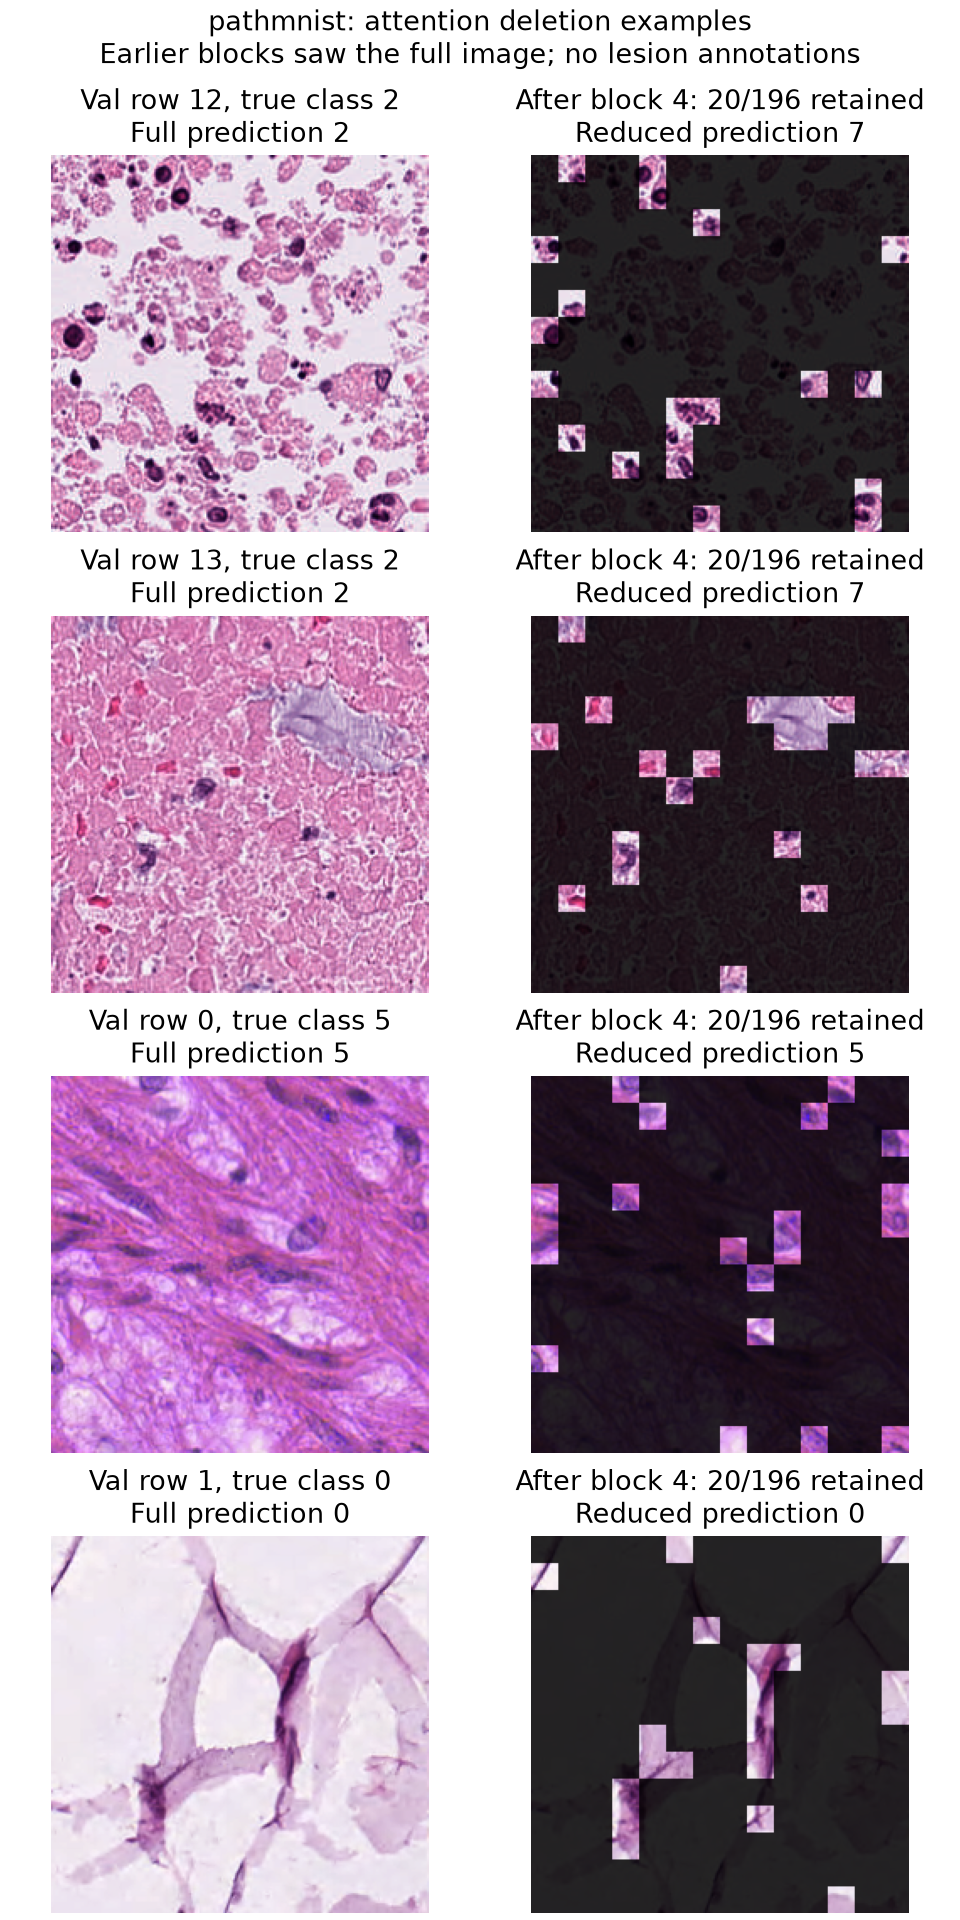
\includegraphics[width=\linewidth]{fig/pathmnist_examples.png}
  \caption{Attention deletion after block 4 on \pathmnist validation images; dimmed patches are removed from later blocks. Illustrative only: without region annotations these overlays cannot validate diagnostic localisation.}
  \label{fig:examples}
\end{figure}

\subsection{Locked test confirmation (Stage 4)}
\label{sec:locked}
\Cref{tab:test} is the main result. Every candidate is the validation winner for its method, frozen before test; recovery rows are paired with equally trained full-token controls. \Cref{fig:paired} shows the per-seed paired differences.

\begin{table*}[t]
  \centering
  \small
  \begin{tabular}{llrrrrrcc}
    \toprule
    Dataset & Policy & Tokens & Reduction & Ref.\ acc.\ & Reduced acc.\ & $\Delta$ mean & Worst LB & NI at 0.5 / 1\,\pp \\
    \midrule
    \pathmnist  & Attention, locked      & 69  & 64.8\% & 96.70 & 95.13 & $-1.57$ & $-2.44$ & no / no \\
    \pathmnist  & EViT-style, locked     & 69  & 64.8\% & 96.70 & 95.06 & $-1.64$ & $-2.59$ & no / no \\
    \pathmnist  & Random, locked         & 49  & 75.0\% & 96.70 & 94.98 & $-1.72$ & $-2.75$ & no / no \\
    \pathmnist  & ToMe-style, locked     & 20  & 89.8\% & 96.70 & 93.94 & $-2.77$ & $-4.28$ & no / no \\
    \pathmnist  & ToMe-style + recovery  & 20  & 89.8\% & 96.12 & 96.30 & $+0.18$ & $-1.12$ & no / no \\
    \midrule
    \dermamnist & Attention, locked      & 147 & 25.0\% & 90.57 & 90.27 & $-0.30$ & $-1.34$ & no / no \\
    \dermamnist & EViT-style, locked     & 147 & 25.0\% & 90.57 & 90.24 & $-0.33$ & $-1.43$ & no / no \\
    \dermamnist & EViT-style + recovery  & 98  & 50.0\% & 90.37 & 90.09 & $-0.28$ & $-1.93$ & no / no \\
    \midrule
    \pneumnist  & ToMe-style, locked     & 69  & 64.8\% & 95.03 & 93.27 & $-1.76$ & $-5.31$ & no / no \\
    \pneumnist  & ToMe-style + recovery  & 49  & 75.0\% & 95.62 & 95.30 & $-0.32$ & $-2.57$ & no / no \\
    \bottomrule
  \end{tabular}
  \caption{Locked test results. Accuracies (\%) and $\Delta$ (\pp) are means over three training seeds; ``Worst LB'' is the smallest conservative simultaneous 95\% lower bound on $\Delta$ among the seeds. Non-inferiority (NI) requires every seed's bound to exceed $-0.5$ (or $-1$)\,\pp. No candidate passed. \TODO{Verify the per-policy reduced accuracies against \texttt{reports/stage4/comparisons.json}; the reference/recovery columns are from the Stage 4 summary.}}
  \label{tab:test}
\end{table*}

\begin{figure}[t]
  \centering
  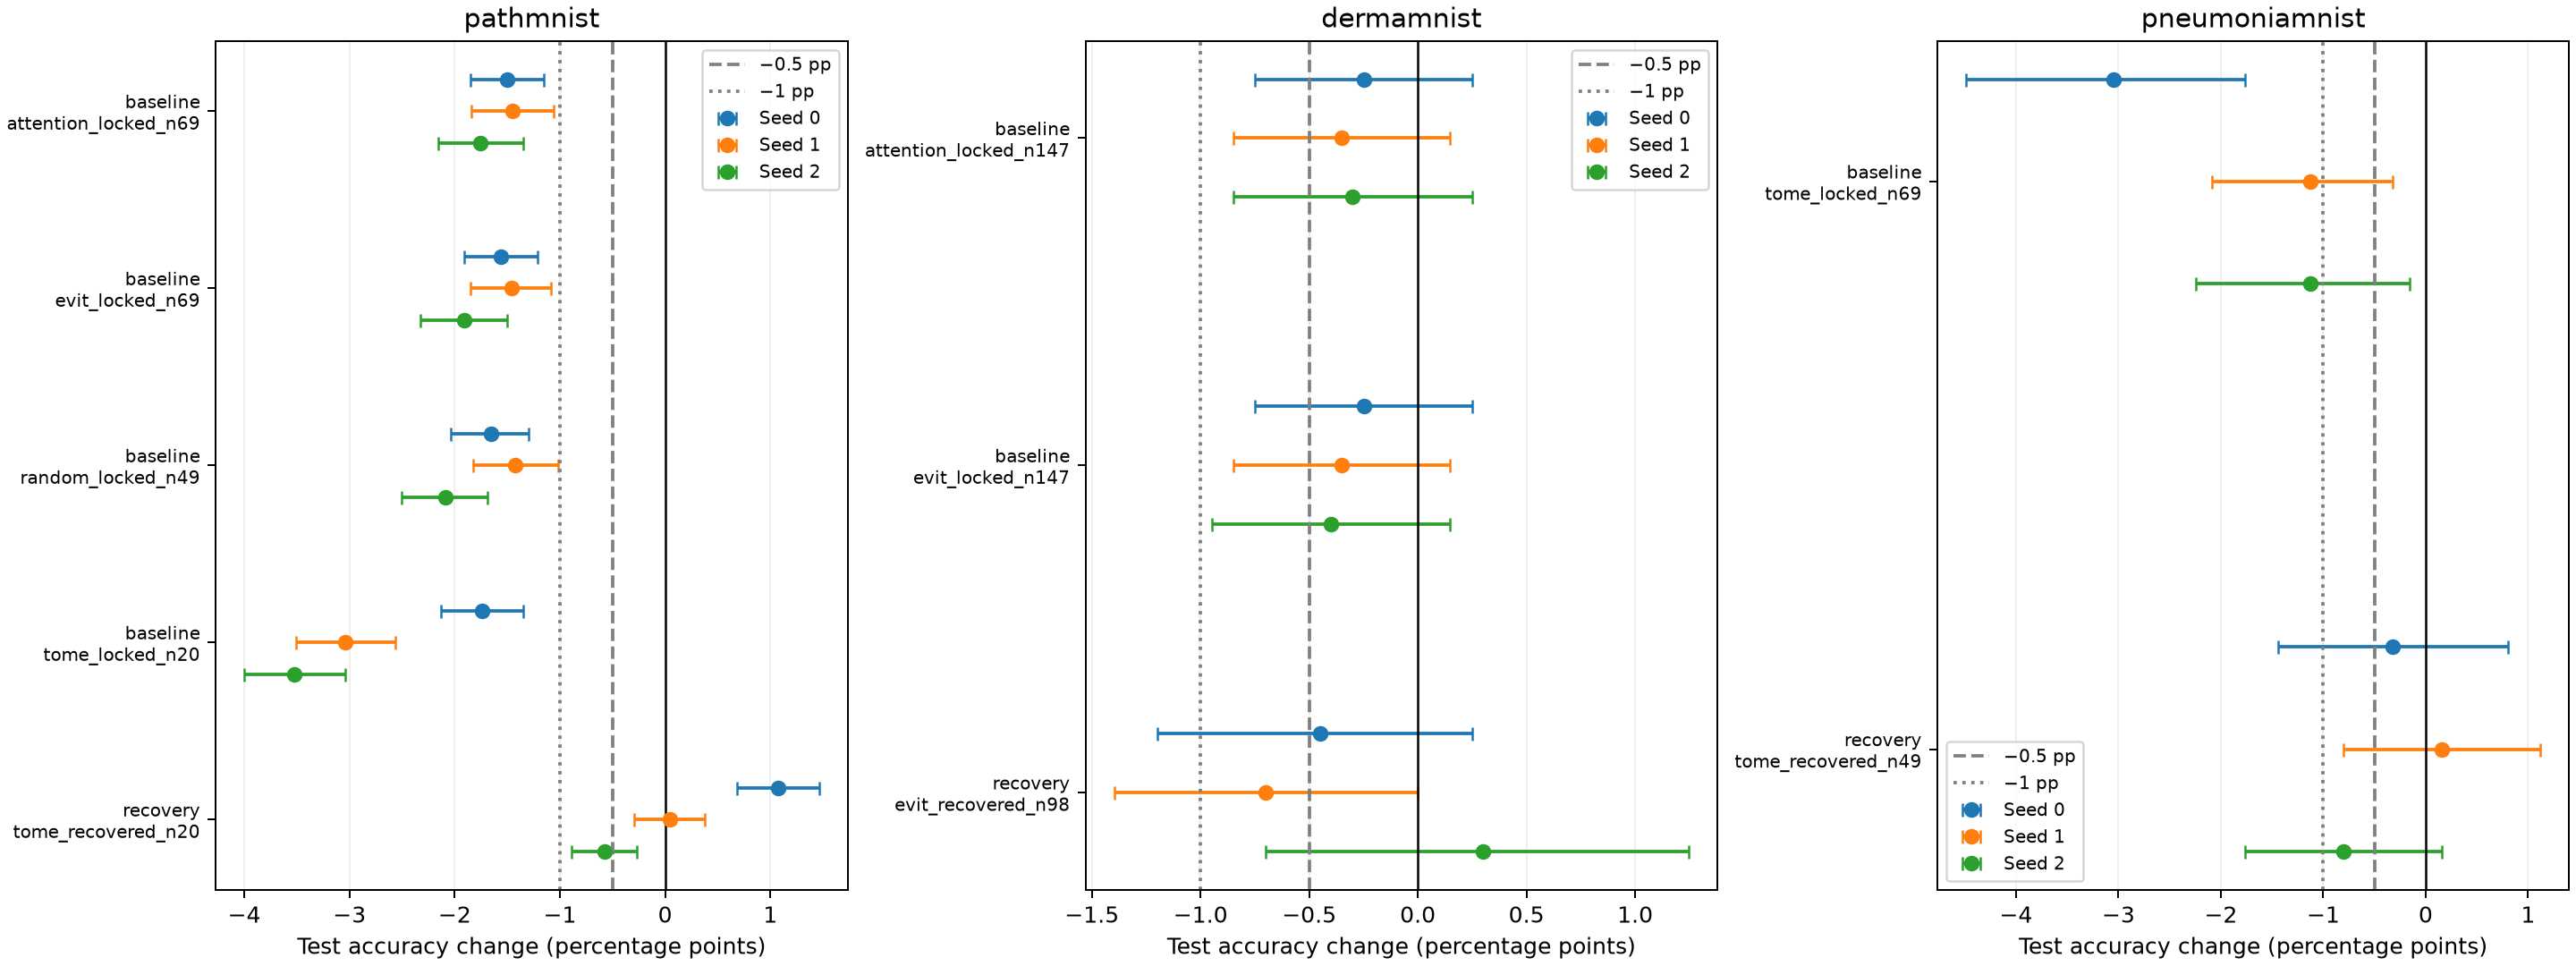
\includegraphics[width=\linewidth]{fig/paired_test_differences.png}
  \caption{Paired test accuracy differences (reduced minus reference) per seed with descriptive bootstrap 95\% intervals. Decisions in \cref{tab:test} use the more conservative simultaneous bounds.}
  \label{fig:paired}
\end{figure}

Three patterns stand out. First, \pathmnist's apparent robustness on validation did not transfer: all four locked policies lost 1.6--2.8\,\pp on a test set drawn from a different centre, and the 20-token merged model lost up to 12.4\,\pp of cancer-associated-stroma recall in one seed. Second, \dermamnist's conservative 147-token policies lost only 0.3\,\pp on average, but the 2{,}005-image test set yields bounds no tighter than $-1.3$\,\pp. Third, recovery helped everywhere, moving mean losses to $-0.3$\,\pp or better, yet seed-to-seed spread (e.g.\ $-0.57$ to $+1.07$\,\pp on \pathmnist) kept at least one bound below the margin in every case. None of the ten candidates established either margin.

\subsection{Compute and measured speed}
\Cref{tab:eff} shows that FLOP reduction and wall-clock gain diverge. Merging to 20 tokens cuts FLOPs by 59\% and raises batch-32 throughput by 75\%, but \emph{increases} batch-1 latency by 22\% because the matching step is not hidden at batch size 1. Only the mild \dermamnist fusion policy improves both. Any claim of ``$k\times$ faster'' for token reduction therefore needs to state the batch size.

\begin{table}[t]
  \centering
  \small
  \setlength{\tabcolsep}{4pt}
  \begin{tabular}{llrrr}
    \toprule
    Dataset & Policy & GFLOPs & Lat.\ (ms, b=1) & img/s (b=32) \\
    \midrule
    \pathmnist  & ToMe 20  & $9.20\!\to\!3.75$ & $2.13\!\to\!2.61$ & $3202\!\to\!5607$ \\
    \dermamnist & EViT 147 & $9.20\!\to\!7.66$ & $2.14\!\to\!2.01$ & $3171\!\to\!3614$ \\
    \pneumnist  & ToMe 69  & $9.20\!\to\!5.19$ & $2.15\!\to\!2.32$ & $3152\!\to\!4538$ \\
    \bottomrule
  \end{tabular}
  \caption{Full $\to$ reduced compute and speed on test inputs for the validation-selected policies without recovery (float32, means over three seeds, overhead of selection/merging included).}
  \label{tab:eff}
\end{table}

\subsection{Fine-tuning method comparison}
\label{sec:ftgrid}
\TODO{Fill from \texttt{outputs/finetune/*/*/seed\_*/training\_summary.json} (scripts/finetune\_grid.sh prints the table) and \texttt{outputs/pruning\_study/summary.md}.} We fine-tune each dataset with the four methods of \cref{sec:finetune} and three seeds (36 runs), then (a) sweep every checkpoint over the full Stage 2 budget grid on test, descriptively, to see whether the adaptation method changes pruning tolerance, and (b) compare full-parameter and LoRA recovery from the same starting checkpoint under the locked recovery budgets, each against its own equally trained control.

\begin{table}[t]
  \centering
  \small
  \setlength{\tabcolsep}{4pt}
  \begin{tabular}{llrrrr}
    \toprule
    Dataset & Method & Train.\ params & Val.\ acc.\ & Time (s) & Mem (GB) \\
    \midrule
    \multirow{4}{*}{\pathmnist}  & Full    & 21.7M & \TODO{} & \TODO{} & \TODO{} \\
                            & Partial & \TODO{} & \TODO{} & \TODO{} & \TODO{} \\
                            & LoRA    & \TODO{} & \TODO{} & \TODO{} & \TODO{} \\
                            & Linear  & \TODO{} & \TODO{} & \TODO{} & \TODO{} \\
    \midrule
    \multirow{4}{*}{\dermamnist} & Full    & \TODO{} & \TODO{} & \TODO{} & \TODO{} \\
                            & Partial & \TODO{} & \TODO{} & \TODO{} & \TODO{} \\
                            & LoRA    & \TODO{} & \TODO{} & \TODO{} & \TODO{} \\
                            & Linear  & \TODO{} & \TODO{} & \TODO{} & \TODO{} \\
    \midrule
    \multirow{4}{*}{\pneumnist}  & Full    & \TODO{} & \TODO{} & \TODO{} & \TODO{} \\
                            & Partial & \TODO{} & \TODO{} & \TODO{} & \TODO{} \\
                            & LoRA    & \TODO{} & \TODO{} & \TODO{} & \TODO{} \\
                            & Linear  & \TODO{} & \TODO{} & \TODO{} & \TODO{} \\
    \bottomrule
  \end{tabular}
  \caption{Adaptation methods: trainable parameters, best validation accuracy (mean over three seeds), optimisation-only training time and peak GPU memory. \TODO{Hardware for these runs.}}
  \label{tab:ftgrid}
\end{table}

\begin{table}[t]
  \centering
  \small
  \setlength{\tabcolsep}{4pt}
  \begin{tabular}{llrrr}
    \toprule
    Dataset & Recovery & Tokens & Test $\Delta$ vs.\ own control & Worst LB \\
    \midrule
    \pathmnist  & Full params       & 20 & \TODO{} & \TODO{} \\
    \pathmnist  & LoRA              & 20 & \TODO{} & \TODO{} \\
    \pathmnist  & LoRA from LoRA FT & 20 & \TODO{} & \TODO{} \\
    \dermamnist & Full params       & 98 & \TODO{} & \TODO{} \\
    \dermamnist & LoRA              & 98 & \TODO{} & \TODO{} \\
    \dermamnist & LoRA from LoRA FT & 98 & \TODO{} & \TODO{} \\
    \pneumnist  & Full params       & 49 & \TODO{} & \TODO{} \\
    \pneumnist  & LoRA              & 49 & \TODO{} & \TODO{} \\
    \pneumnist  & LoRA from LoRA FT & 49 & \TODO{} & \TODO{} \\
    \bottomrule
  \end{tabular}
  \caption{Recovery under the locked budgets with full-parameter versus LoRA-only updates, each paired with an equally trained full-token control. \TODO{Fill from outputs/pruning\_study/summary.md.}}
  \label{tab:recovery}
\end{table}

\section{Discussion}
\label{sec:discussion}

\paragraph{What transferred, and what did not.}
The ImageNet picture of token reduction, a smooth accuracy-compute trade-off with a comfortable 30--50\% sweet spot, survives on \pathmnist, where tissue texture is highly redundant, and largely fails on \dermamnist, where no deletion budget beyond 25\% qualified even on validation. The ordering of methods also changes: attention-ranked deletion, the basis of EViT, is not reliably better than random deletion here (H2), while merging, which preserves a summary of every token, is the only mechanism that reached aggressive budgets on two datasets (H3). The depth ablation gives a practical rule: removing tokens before any attention has mixed information is far more harmful than removing the same number after four blocks, even though the former saves more compute (H4).

\paragraph{The validation-to-test gap.}
Our central negative result is that budgets which were safe on validation for all three seeds did not establish non-inferiority on test. Part of this is real degradation (\pathmnist, where the test set comes from a different centre) and part is precision: \pneumnist has 624 test images, so the conservative bound cannot resolve a 0.5\,\pp margin even when the point estimate is close to zero. Both outcomes argue against reporting validation-selected pruning rates as deployable limits, which is the common practice in the literature we build on. Recovery training is the most promising lever: two epochs reduced the mean loss on every dataset and turned the \pathmnist loss into a small gain, but seed variation kept the bounds below the margin. Whether LoRA-only recovery, which updates under 1\% of the weights, can match full recovery is addressed in \cref{sec:ftgrid}. \TODO{Update once recovery results are in.}

\paragraph{Class-level harm.}
Aggregate accuracy hid recall drops of 6--12\,\pp on a single class in individual seeds (H5). The affected classes were sometimes the clinically relevant ones (cancer-associated stroma) and sometimes small-support classes where one or two images move the number. Any deployment criterion would need a separate sensitivity margin; we deliberately asserted none.

\paragraph{Limitations.}
The study covers one backbone size, one pretraining regime, three 2D classification benchmarks and a five-point budget grid. EViT and ToMe are controlled adaptations, so our conclusions concern the mechanisms (summary preservation, merging) rather than the published systems. Intervals are image-level and ignore within-patient correlation. Latency reflects an unoptimised research implementation; merging in particular adds batch-1 overhead that a fused kernel would remove. Finally, the selected validation maxima are grid maxima, not population limits, and we did not retune anything after seeing test results.

\section{Conclusion}
We measured how far token reduction and parameter-efficient adaptation can be pushed on a medical \deit under a protocol that locks every decision before test inference. The tolerable reduction is dataset-specific, merging beats deletion, depth matters more than count, and small validation-safe losses do not survive conservative held-out confirmation. We hope the locked-test methodology, more than any particular number, is what carries over to future work on efficient medical vision transformers. \TODO{Add the fine-tuning/LoRA takeaway.}

{
    \small
    \bibliographystyle{ieeenat_fullname}
    \bibliography{main}
}

% Supplementary material does not count toward the 4-page limit.
% \clearpage
% \input{sec/X_suppl}

\end{document}
